This methodology performs a series of non-linear time history analyses (NLTHA) over one or multiple single degree of freedom (SDoF) systems. In order to determine the structural capacity of the system(s) under analysis, it is necessary to identify the relationship between the base shear and roof displacement (i.e. pushover curve). This curve can be further modified in order to obtain the curve corresponding to an equivalent SDoF, or capacity curve. It is typically assumed that the fundamental mode of vibration corresponds with the predominant response of the structure. Under this hypothesis, the capacity curve usually represents the first mode of response of the structure. This is usually valid for buildings with fundamental periods of vibration up to approximately 1.0 s. Otherwise, higher modes should be taken into account. Along with the capacity curve, it is necessary to specify either the mass or the fundamental period of vibration of the SDoF system.\\

On the other hand, the demand is represented by a set of ground motion records. The response of each structure is given by the solution of the equation of motion for an inelastic SDoF under earthquake excitation:

\begin{equation}
m\ddot{u}(t) + c\dot{u}(t) + ku(t) = p(t)
\end{equation}

Where $u$, $\dot{u}$ and $\ddot{u}$ stand for the displacement, velocity and acceleration, respectively, over time ($t$), and $p$ represents an external excitation. In this method, the behaviour of the SDoF is modelled by a capacity curve that must follow the structure illustrated in Figure \ref{fig:backbone}.

\begin{figure}[htb]
  \centering
      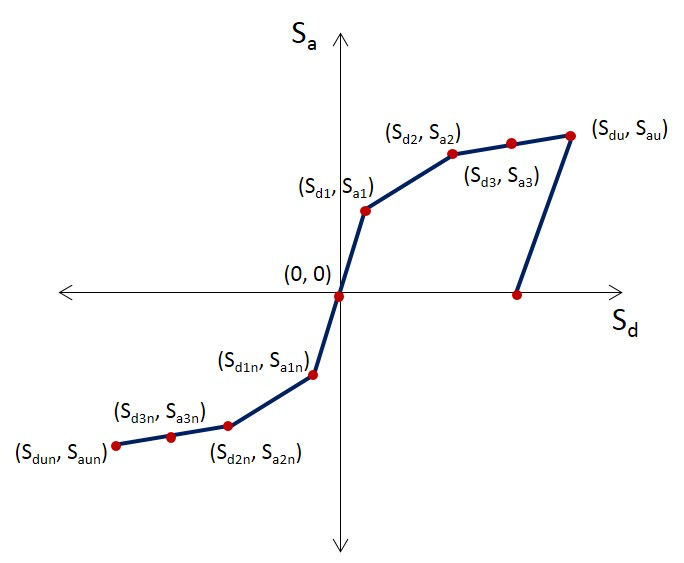
\includegraphics[width=9cm]{figures/backbone_curve.png}
  \caption{Representation of the capacity curve required to represent the structural capacity of the SDoF system.}
  \label{fig:backbone}
\end{figure}

Six relevant points should be defined in this curve. The first one corresponds to the origin, $(0, 0)$. The next point, $(S_{dy}, S_{ay})$, corresponds to the yielding point of the structure, i.e. the point beyond which the structure no longer displays an elastic behaviour. The following two points are defined as any two intermediate points between the yield point and the ultimate point which can be used to represent particular structural properties, such as reduction of stiffness due to collapse of infill panels or softening behaviour due to P-delta effects. The ultimate point $(S_{du}, S_{au})$ corresponds to the point of maximum displacement of the structure. Finally, the last point $(S_{du}, 0)$ is just a control point to define the hysteretic model, in case degradation is considered in the analysis. For the purposes of the RMTK, the first five points must be provided as input. The nonlinear time history analysis are performed using the open-source software for structural analysis OpenSees \citep{McKennaEtAl2000}. It is important to understand the GEM Foundation does not have authorization to distribute this tool, and therefore in order to use this methodology, users are expected to download OpenSEES (http://opensees.berkeley.edu/), and allocate it in the appropriate folder (\verb=vulnerability/derivation_fragility/NLTHA_on_SDOF=).\\

In order to use this methodology, it is necessary to load one or multiple capacity curves and a set of ground motion records, as explained in Sections~\ref{subsec:cap_curves} and \ref{subsec:gmrs}, respectively. Then, it is necessary to specify a damage model using the parameter \verb=damage_model= (see Section~\ref{subsec:dmg_model}). The damping ratio must be defined using the parameter \verb=damping=, and if structural degradation should be considered in the analysis, it is necessary to set the parameter \verb=degradation= to \verb=True=. After importing the module \verb=NLTHA_on_SDOF=, it is possible to calculate the distribution of structures across the set of damage states for each ground motion record using the following command:

\begin{Verbatim}[frame=single, commandchars=\\\{\}, samepage=true]
PDM, Sds = NLTHA_on_SDOF.calculate_fragility(capacity_curves,gmrs,...
damage_model,damping)
\end{Verbatim}

Where \verb=PDM= (i.e. probability damage matrix) represents a matrix with the number of structures in each damage state per ground motion record, and \verb=Sds= (i.e. spectral displacements) represents a matrix with the maximum displacement (of the equivalent SDoF) of each structure per ground motion record. The variable PDM can then be used to calculate the mean fragility model as described in Section \ref{subsec:derive_fragility}.